\documentclass[crop,tikz]{standalone}                 
\usepackage{physics}

\makeatletter                                                                                        

\newcommand{\sq}[1]{\frac{1}{\sqrt{#1}}}

\begin{document}

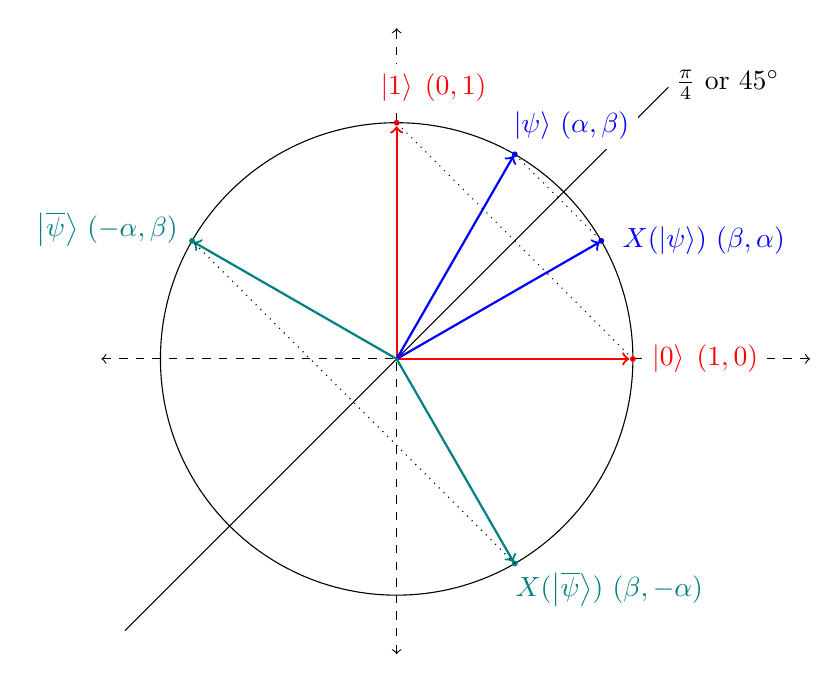
\begin{tikzpicture}[scale=1.5]                                                                          
\usetikzlibrary{positioning}
%\draw [dashed,gray, step=2cm] (-2.30,-2.30) grid ( 2.30, 2.30);

% Axes
\draw [-] (-2.30,-2.30) -- ( 2.30, 2.30);
\draw [<->, dashed] (0,-2.5) -- (0,2.8);
\draw [<->, dashed] (-2.5, 0) -- (3.5,0);

% Circle
\draw[] (0cm,0cm) circle(2.00cm);                                                                 

% Point ket-1
\filldraw[red] (0.00,2.00) circle (0.02cm);
\node [fill=white,text=red] (ket1) at ( 0.00, 2.30) {$\ket{1}$};
\node [red]             (al) at ( 0.50, 2.30) {$(0,1)$};
\draw [->,thick,red] (0,0) -- (0.00, 1.97);

% Point ket-0
\filldraw[red] ( 2.00, 0.00) circle (0.02cm);
\node [fill=white,text=red] (ket2) at ( 2.30, 0.00) {$\ket{0}$};
\node [fill=white, text=red]             (al) at ( 2.80, 0.00) {$(1,0)$};
\draw [->,thick,red] (0,0) -- (1.97, 0.00);

% Point ket-psi
\filldraw[blue] ( 1.00, 1.732) circle (0.02cm);
\node [fill=white,text=blue] (ket3) at ( 1.48, 1.976) {$\ket{\psi}$  $(\alpha,\beta)$};
\draw [->,thick,blue] (0,0) -- (0.99, 1.72);

% Point not-ket-psi
\filldraw[blue] (1.732, 1.00) circle (0.02cm);
\node [fill=white,text=blue] (ket4) at ( 2.6, 1.00) {$X(\ket{\psi})$  $(\beta, \alpha)$};
\draw [->,thick,blue] (0,0) -- (1.72, 0.99);

% Point ket-psi-prime
\filldraw[teal] (-1.732, 1.00) circle (0.02cm);
\node [text=teal] (ket5) at (-2.45, 1.10) {$\ket{\overline{\psi}}$  $(-\alpha,\beta)$};
\draw [->,thick,teal] (0,0) -- (-1.72, 0.99);

% Point not-ket-psi-prime
\filldraw[teal] (1.00, -1.732) circle (0.02cm);
\node [text=teal] (ket6) at (1.80,-1.95) {$X(\ket{\overline{\psi}})$  $(\beta,-\alpha)$};
\draw [->,thick,teal] (0,0) -- (0.99,-1.72);

% Reflection Lines
\draw [-,dotted] ( 2.00, 0.00) -- (0.00,2.00);
\draw [-,dotted] ( 1.00, 1.732) -- (1.732, 1.00);
\draw [-,dotted] ( 1.00,-1.732) -- (-1.732, 1.00);

% Angle
\node [] (angle) at ( 2.80, 2.32) {$\frac{\pi}{4}$ or $45^{\circ}$}; 

\end{tikzpicture}                                                                                    

\end{document}
